\documentclass[12pt,twocolumn,landscape,UTF8,twoside]{ctexart}
\usepackage[utf8]{inputenc}

\usepackage[paperwidth=36.8cm,paperheight=26cm,
top=2cm,bottom=2cm,right=2cm,left=3.cm,
columnsep=1.5cm]{geometry}
\columnseprule=.4pt

\usepackage{bbding}
\usepackage{amsmath}
\usepackage{amsfonts}
\usepackage{amssymb}
\usepackage{wasysym}
\usepackage{makeidx}

\usepackage{graphicx}
\usepackage{setspace}
\usepackage{tabu}
\usepackage{paralist}
\usepackage{lastpage}
\usepackage{enumerate} 

\usepackage{fancyhdr}
\renewcommand{\headrulewidth}{0pt}
\pagestyle{fancy}
\fancyfoot[CO,CE]{第~\thepage~页~~共~\pageref{LastPage}~页}
\fancyhead[RE]{\leavevmode\vbox to0pt{
		\vss\rlap{\putzdxx }\vskip -26cm }} %奇数页眉的右边                       
\fancyhead[LO]{\leavevmode\vbox to0pt{
		\vss\rlap{\putzdx }\vskip -26cm }} %偶数页眉的左边 

\newsavebox{\zdxa}%装订线

\sbox{\zdxa}
{\parbox{27cm}{\centering \heiti \hspace{1cm}
		系~部:\underline{\makebox[30mm][c]{}}~~~ 班~级:\underline{\makebox[45mm][c]{}}~~~ 姓~名:\underline{\makebox[30mm][c]{}}~~~ 学~号:\underline{\makebox[30mm][c]{}} \\
		\vspace{1mm}
%		请在所附答题纸上空出密封位置。并填写试卷序号、班级、学号和 姓名\\
		%答题时学号
%		\vspace{1mm}
	  \dotfill{} 〇 \dotfill{} 密\dotfill{}封\dotfill{}线\dotfill{}〇\dotfill{} \\
}}
\newsavebox{\zdxb}%装订线
\sbox{\zdxb}
{\parbox{27cm}{\centering \heiti
		\vspace{30mm}
		\vspace{1mm}
		\dotfill{} 〇 \dotfill{}密\dotfill{}封\dotfill{}线\dotfill{}〇\dotfill{} \\
}}

\newcommand{\putzdx}{
		\hspace{-1.7cm}\parbox{1cm}{\vspace{-1.5cm}
			\rotatebox[origin=c]{90}{
				\usebox{\zdxa}
		}}
}
\newcommand{\putzdxx}{
	\hspace{0.3cm}\parbox{1cm}{\vspace{-1.5cm}
		\rotatebox[origin=c]{-90}{
			\usebox{\zdxb}
	}}
}


\usepackage{ifthen}

%选择题选项命令 \xx \xxiii \xxv \xxvi
\newlength{\la}
\newlength{\lb}
\newlength{\lc}
\newlength{\ld}
\newlength{\lee}
\newlength{\lf}
\newlength{\lhalf}
\newlength{\lquarter}
\newlength{\lmax}
\newcommand{\xx}[4]{\\[.5pt]%  
	\settowidth{\la}{A、#1~~~}  
	\settowidth{\lb}{B、#2~~~}
	\settowidth{\lc}{C、#3~~~}  
	\settowidth{\ld}{D、#4~~~}  
	\ifthenelse{\lengthtest{\la > \lb}}
	{\setlength{\lmax}{\la}}{\setlength{\lmax}{\lb}}  
		\ifthenelse{\lengthtest{\lmax < \lc}}  {\setlength{\lmax}{\lc}}  {}  \ifthenelse{\lengthtest{\lmax < \ld}}  {\setlength{\lmax}{\ld}}  {} 
	    \setlength{\lhalf}{0.5\linewidth} 
	    \setlength{\lquarter}{0.25\linewidth}
	    \ifthenelse{\lengthtest{\lmax > \lhalf}}  
	    {\noindent{}A、#1 \\ B、#2 \\ C、#3 \\ D、#4 }  {  \ifthenelse{\lengthtest{\lmax > \lquarter}}  
	    	{\noindent
	    	 \makebox[\lhalf][l]{A、#1~~~}% 
	    	 \makebox[\lhalf][l]{B、#2~~~}\\%
	    	 \makebox[\lhalf][l]{C、#3~~~}%
	    	 \makebox[\lhalf][l]{D、#4~~~}}% 
    		 {\noindent\makebox[\lquarter][l]{A、#1~~~}% 
    		 \makebox[\lquarter][l]{B、#2~~~}%     
    		 \makebox[\lquarter][l]{C、#3~~~}%      
    		 \makebox[\lquarter][l]{D、#4~~~}}
    	 }}
     
\newcommand{\xxiii}[3]{\\[.5pt]%  
	\settowidth{\la}{A、#1~~~}  
	\settowidth{\lb}{B、#2~~~}
	\settowidth{\lc}{C、#3~~~}  
	\ifthenelse{\lengthtest{\la > \lb}}
	{\setlength{\lmax}{\la}}{\setlength{\lmax}{\lb}}  
	\ifthenelse{\lengthtest{\lmax < \lc}}  {\setlength{\lmax}{\lc}}  {}  
	\setlength{\lhalf}{0.5\linewidth} 
	\setlength{\lquarter}{0.25\linewidth}
	\ifthenelse{\lengthtest{\lmax > \lhalf}}  
	{\noindent{}A、#1 \\ B、#2 \\ C、#3 }  {  \ifthenelse{\lengthtest{\lmax > \lquarter}}  
		{\noindent
			\makebox[\lhalf][l]{A、#1~~~}% 
			\makebox[\lhalf][l]{B、#2~~~}\\%
			\makebox[\lhalf][l]{C、#3~~~}}% 
		{\noindent
			\makebox[\lquarter][l]{A、#1~~~}% 
			\makebox[\lquarter][l]{B、#2~~~}%     
			\makebox[\lquarter][l]{C、#3~~~}}
}}

\newcommand{\xxv}[5]{\\[.5pt]%  
	\settowidth{\la}{A、#1~~~}  
	\settowidth{\lb}{B、#2~~~}
	\settowidth{\lc}{C、#3~~~} 
	\settowidth{\ld}{D、#4~~~}  
	\settowidth{\lee}{E、#5~~~}   
	\ifthenelse{\lengthtest{\la > \lb}}
	{\setlength{\lmax}{\la}}{\setlength{\lmax}{\lb}}  
	\ifthenelse{\lengthtest{\lmax < \lc}}  {\setlength{\lmax}{\lc}}  {} 
	\ifthenelse{\lengthtest{\lmax < \ld}}  {\setlength{\lmax}{\ld}}  {} 
	\ifthenelse{\lengthtest{\lmax < \lee}}  {\setlength{\lmax}{\lee}}  {} 
	\setlength{\lhalf}{0.5\linewidth} 
	\setlength{\lquarter}{0.25\linewidth}
	\ifthenelse{\lengthtest{\lmax > \lhalf}}  
	{\noindent{}A、#1 \\ B、#2 \\ C、#3 \\ D、#4 \\ E、#5}  {  \ifthenelse{\lengthtest{\lmax > \lquarter}}  
		{\noindent
			\makebox[\lhalf][l]{A、#1~~~}% 
			\makebox[\lhalf][l]{B、#2~~~}\\%
			\makebox[\lhalf][l]{C、#3~~~}%
		    \makebox[\lhalf][l]{D、#4~~~}\\%
		    \makebox[\lhalf][l]{E、#5~~~}}% 
		{\noindent
			\makebox[\lquarter][l]{A、#1~~~}% 
			\makebox[\lquarter][l]{B、#2~~~}%     
			\makebox[\lquarter][l]{C、#3~~~}%
		    \makebox[\lquarter][l]{D、#4~~~}\\%
	        \makebox[\lquarter][l]{E、#5~~~}}
}}

\newcommand{\xxvi}[6]{\\[.5pt]%  
	\settowidth{\la}{A、#1~~~}  
	\settowidth{\lb}{B、#2~~~}
	\settowidth{\lc}{C、#3~~~} 
	\settowidth{\ld}{D、#4~~~}  
	\settowidth{\lee}{E、#5~~~}
	\settowidth{\lf}{E、#6~~~}     
	\ifthenelse{\lengthtest{\la > \lb}}
	{\setlength{\lmax}{\la}}{\setlength{\lmax}{\lb}}  
	\ifthenelse{\lengthtest{\lmax < \lc}}  {\setlength{\lmax}{\lc}}  {} 
	\ifthenelse{\lengthtest{\lmax < \ld}}  {\setlength{\lmax}{\ld}}  {} 
	\ifthenelse{\lengthtest{\lmax < \lee}}  {\setlength{\lmax}{\lee}}  {}
    \ifthenelse{\lengthtest{\lmax < \lf}}  {\setlength{\lmax}{\lf}}  {}  
	\setlength{\lhalf}{0.5\linewidth} 
	\setlength{\lquarter}{0.25\linewidth}
	\ifthenelse{\lengthtest{\lmax > \lhalf}}  
	{\noindent{}A、#1 \\ B、#2 \\ C、#3 \\ D、#4 \\ E、#5 \\ F、#6}  {  \ifthenelse{\lengthtest{\lmax > \lquarter}}  
		{\noindent
			\makebox[\lhalf][l]{A、#1~~~}% 
			\makebox[\lhalf][l]{B、#2~~~}\\%
			\makebox[\lhalf][l]{C、#3~~~}%
			\makebox[\lhalf][l]{D、#4~~~}\\%
			\makebox[\lhalf][l]{E、#5~~~}%
		    \makebox[\lhalf][l]{F、#6~~~}}% 
		{\noindent
			\makebox[\lquarter][l]{A、#1~~~}% 
			\makebox[\lquarter][l]{B、#2~~~}%     
			\makebox[\lquarter][l]{C、#3~~~}%
			\makebox[\lquarter][l]{D、#4~~~}\\%
			\makebox[\lquarter][l]{E、#5~~~}%
		    \makebox[\lquarter][l]{F、#6~~~}}%
}}

%填空题画线  \tk
%\newcommand{\tk}[2][2.5]{\; \underline{\hspace{#1 cm} \hphantom{#2} \hspace{#1 cm} } \, }


%判断题后面加括号
\newcommand{\pd}[2][1]{\nolinebreak\dotfill\mbox{\raisebox{-1.8pt}
		{$\cdots$}(\makebox[#1 cm][c]{
		\ifthenelse{\boolean{print}}
		{\ifthenelse{\equal{#2}{t}}{\Checkmark}{\XSolid}}
		{}
		})}}

\newboolean{print}
\setboolean{print}{true}

\usepackage{ulem}
\newcommand{\tk}[2][0.5]{\;\uline{ 
		\hspace*{#1 cm}
		 \ifthenelse{\boolean{print}}{#2}{\hphantom{#2}}  
	 	 \hspace*{#1 cm}
 	 } }



%\setboolean{print}{true}
%\setboolean{print}{false} %是否打印答案

\author{高星}

\begin{document}
\noindent	
	
\begin{spacing}{1.5}
		\begin{center}
			\zihao{3} \heiti 
				湖南潇湘技师学院~~湖南九嶷职业技术学院
				
				\underline{~2017~-- 2018 }\,学年 \hspace{1cm} 第\,\underline{~1~}\,学期
				
				\underline{~《 数铣编程与操作》~}\,期中考试试题\,\underline{~A~}\,卷 (\,时间: \underline{~90 分钟~}\,)

\zihao{-4} \songti \vspace{2mm}
\begin{tabu} to 0.45\textwidth {|X[2,c]|X[1,c]|X[1,c]|X[1,c]|X[1,c]
	|X[1,c]|X[1,c]|X[1,c]|X[1,c]|X[1,c]
|X[1,c]|X[2,c]|}
	\hline 
	题\hfill 号&一&二&三&四&五&六& 七&八&九&十&总\hfill 分\\ 
	\hline 
	得\hfill 分&  &  &  &  &  &  &  &  &  &  &  \\ 
	\hline 
	评\hfill 卷\hfill 人&  &  &  &  &  &  &  &  &  &  &  \\ 
	\hline 
\end{tabu} 
\end{center}
\end{spacing}
\vspace{-10pt}\zihao{5} 
\begin{spacing}{1.3}
	\begin{enumerate} [1、]
		\item[\heiti 一、] {\heiti 填空题(每空0.5分,共20分)}
		\item 数控机床由 \tk{输入输出设备}、\tk{数控装置}、\tk{伺服系统}、\tk{机床本体} 和其它辅助装置等组成。
		
		\item 数控机床按运动控制方式可分为\tk{点位控制数控机床}、直线控制数控机床和	\tk{连续控制数控机床}。
		
		\item 数控编程一般有\tk{手工编程}和\tk{自动编程}两种方法。
		
		\item 在加工中心中,F指令用于指定\tk{进给速度} ,S指令用于指定\tk{主轴转速},T指令用于指定\tk{加工刀具};其中F100表示\tk{进给速度为100mm/min},S800表示\tk{主轴转速为800r/min}。
		
		\item \tk{键槽}铣刀有两个刀齿,端面刃延至刀具中心,即像立铣刀又像钻头,可直接进行轴向加工。
		
		\item 加工中心是一种带\tk{刀库}和\tk{自动换刀装置}的数控机床。

		\item 用G54设定工件坐标系时,可用多种方法找到工件坐标系原点在 \tk{机床}坐标系中的坐标,并把其坐标值输入到相应的参数中。

		\item 每脉冲使机床移动部件产生的位移称\tk{脉冲当量}  		。

		\item 在数控编程时,使用\tk{刀具半径}指令后,就可以按工件的轮廓尺寸进行编程,而不需按照刀具的中心线运动轨迹来编程。
		
		\item 在铣削零件的内外轮廓表面时,为防止在刀具切入、切出时产生刀痕,应沿轮廓\tk{切线}方向切入、切出,而不应法线方向切入、切出。

		\item 数控机床中的标准坐标系采用\tk{右手笛卡尔直角坐标系},并规定使刀具与工件之间距离\tk{增大}的方向为正方向。

		\item 在Fanuc上调用5次O1111子程序的指令是\tk{M98 P51111},在Siemens上调用5次L11子程序的指令是\tk{L11 P5}	。

		\item 粗加工时,应选择\tk{较大}的背吃刀量、进给量,\tk{较少}的切削速度。
		精加工时,应选择\tk{较少}的进给量,较\tk{较大}的切削速度(较大/较少)。
		
		\item 铣削进给速度F与铣刀刃数Z、主轴转速S、每齿进给量Fz的关系是	\tk{$F=Fz\times S\times Z$}		。
		
		\item 根据刀具回转切入方向与工件进给方向之间的关系不同,有\tk{顺}铣和\tk{逆}		铣之分。
		
		\item 数控机床在开机后,须进行回零操作,使X、Y、Z各坐标轴运动回到\tk{机床坐标系零点}。
		
		\item 常见的切入、切出方式有三种分别为从延长线上切入、切出,从切线上切入、切出,\tk{法线切入、切出}。
		
		\item 在程序中设置进给速度为F150,若进给倍率打到80,则实际进给速度约为	\tk{120mm/min}。
		
		\item 在主程序中使用M99,则返回到\tk{主程序开头}。

		\item 若采用圆弧切入、切出工件,则刀具半径补偿值必须\tk{少于}切入、切出圆弧半径。

		\item 用6.2的刀补加工 $\diameter 80^{~\;0}_{-0.04}$ 的圆,经测量后其尺寸为\diameter 80.42,侧精加工刀补为\tk{5.98}。

		\item 在自动运行中,打开\tk{单段}功能,可以使程序一段一段的运行,即按下循环启动一次,执行一条数控指令。

		\item 按下进给保持,可使程序运行\tk{暂停运行}		。

		\item 若机床移动部件超出其运动的极限位置(软件行程限位或机械限位),则系统出现\tk{超程}报警。

		\item 在设定刀具半径补偿值时,可在几何和磨损两区域同时设定数值,则补偿值等于几何值与磨损值之\tk{和}。

		\item 若手轮的进给倍率旋钮选择x100,转动手轮5个脉冲,则机床移动\tk{0.5}mm。
		

\item[\heiti 二、] {\heiti 选择题(每题0.5分,共16分)}	
		
\item 沿刀具前进方向观察,刀具偏在工件轮廓的左边上\tk{B}指令。
\xx{G40}{G41}{G42}{G43}	
\item 沿刀具前进方向观察,刀具偏在轮廓的右边是\tk{C}指令。
\xx{G40}{G41}{G42}{G43}	
\item 下面指令中属于非模态指令的是\tk{C}。
\xx{G90}{G2	}	{G4}	{G99}
\item 圆弧插补指令 G17 G3 X\_\_ Y\_\_ R\_\_ F\_\_中的XY表示圆弧的\tk{B}	。
\xx{起点坐标}	{终点坐标}	{圆心坐标}	{圆心相对于起点的值}
\item G00指令与下列的\tk{D}指令不是同一组的。
\xx{G1}		{G2}	{G3}	{G4}
\item 确定数控机床的坐标轴时,一般应先确定\tk{C}	。
\xx{X轴}	{Y轴} {Z轴}		{U轴}
\item 数控铣床的默认加工平面是\tk{A}。
\xxiii{XY平面}		{ZX平面}		{YZ平面}		
\item 开环控制系统用于\tk{A}数控机床上。
\xxiii{经济型}		{中、高档}		{精密}
\item 加工中心与数控铣床的主要区别是\tk{C}	。
\xxiii{数控系统复杂程序不同}	{机床精度不同}	{有无自动换刀系统}
\item 加工中心中的F功能的默认单位是\tk{B}。
\xx{m/min}	{mm/min}	{mm/r}	{m/r}
\item 在数控机床坐标系中平行机床主轴的直线运动为	\tk{C}。
\xxiii{X轴}	{Y轴}{Z轴}
\item 辅助功能中与主轴有关的M指令为\tk{A}。
\xx{M5} {M6}{M9}{M7}
\item “CNC”的含义是	\tk{B}。
\xxiii{数字控制}{计算机数字控制}{网络控制}
\item 在“机床锁定”(FEED HOLD)方式下,进行自动运行,	\tk{A}功能被锁定。
\xxiii{进给}	{主轴} {刀具功能}
\item 在CRT/MDI面板的功能键中,显示机床现在位置的键是\tk{A}。
\xx{POS}	{PRGRM}	{OFSET}	{SYSTEM}
\item 在数控机床工作时,当发生任何异常现象需要紧急处理时应启动\tk{C}。
\xxiii{程序停止功能}	{暂停功能}	{急停功能}
\item 准备功能G90表示的功能是	\tk{C}。
\xx{预置功能}	{固定循环}	{绝对尺寸}	{增量尺寸}
\item 若铣削速度为75m/min,铣刀直径为80mm,则铣刀的转速为\tk{B}r/min。
\xx{258}{298}	{358}	{398}
\item 程序结束时,以何种指令表示\tk{C}。
\xx{M0}	{M1}{M2}{M3}
\item 数控机床的旋转轴之一B轴是绕\tk{B}直线轴旋转的轴。
\xx{X轴}	{Y轴}{Z轴}{W轴}
%\item Fanuc加工中心系统中,用于深孔加工的指令是		。
%\xx{G73}{G81}{G82}{G85}
\item Fanuc上子程序结束的指令为\tk{C}。
\xx{G99}	{G98}	{M99}	{M98}
\item 在Fanuc系统中,在主程序中调用子程序O1000,其正确的指令是\tk{C}		。
\xx{M98 O1000}		{M99 O1000}		{M98 P1000}		{G98 P1000}
\item 通过刀具当前位置来设定工件坐标系时用\tk{C}指令实现。
\xx{G54}		{G55}		{G92}		{G52}
\item 某加工程序中的一个程序段为:N30 G91 G18 G2 X30.0 Y35.0 I30.0 F200 
该段程序的错误在于\tk{B}。
\xx{不应该用G91}	{不应该用G18}	{不应该用N30}	{不应该用G2}
\item 若要使刀具中心远离编程轮廓,则刀补的绝对值\tk{A}。
\xxiii{增大}	{减少}	{不变}	
\item 若要使刀具中心靠近编程轮廓,则刀补的绝对值\tk{B}。
\xxiii{增大}	{减少}	{不变}	
\item 下面使用刀补正确的是\tk{A}。
\xx{G17 G41 G1 X10.0 Y10.0 D1 F200}
{G17 G41 G1 Z-5.0 D1 F200}
{G17 G41 G2 X20.0 Y20.0 R20.0 D1 F200}
{G17 G42 G0 X10.0 Y10.0 F200}
\item 用6.2的刀补加工$\diameter 100^{+0.04}_{~\; 0}$的外圆,经测量其值为 \diameter 100.46,侧精加工刀补为\tk{C}	。
\xx{6.0}	{6.43}	{5.98}	{5.97}
\item 用6.2的刀补加工$\diameter 100$的外圆,经测量其值为 \diameter 100.46,侧精加工刀补为\tk{D}	。
\xx{6.0}	{6.43}	{5.98}	{5.97}
\item 用增量的方式、螺旋下刀一周的指令为\tk{A}。
\xx{G17 G91 G2 X0 Y0 Z-4.0 I20.0 J0}
{G17 G91 G2 X20.0 YO Z-4.0 I20.0 J0}
{G17 G91 G2 X0 Y0 Z-4.0 R20.0}
{G17 G91 G2 X0 Y0 Z-4.0 R-20.0}
\item 加工狭长的槽,可用立铣刀\tk{B}。
\xxiii{直接下刀}{斜线下刀}{螺旋下刀}	
\item 刀具所在位置的坐标为(-20,0),以坐标系原点为中心,逆时针圆弧插补到(0,20)的指令为\tk{B}。
\xx{G17 G3 X0 Y20.0 R20.0}	{G17 G3 X0 Y20.0 I20.0 J0}
{G17 G3 X0 Y20.0 I0 J20.0}		{G17 G3 X-20.0 Y0 R-20.0}				
\item[\heiti 三、] { \heiti 判断题(每题0.5分,共20分)}
		
\item 圆弧插补中,对于整圆,其起点和终点相重合,用R编程无法定义,所以只能用圆心坐标编程。\pd{t}
\item 用数显技术改造后的机床就是数控机床。\pd{f}
\item G代码可以分为模态G代码和非模态G代码。\pd{t}
\item G0和G1指令都能使机床坐标轴准确到位,因此它们都是插补指令。\pd{f}
\item 圆弧插补用半径编程时,当圆弧所对应的圆心角大于180度时半径取负值。\pd{t}
\item 点位控制系统不仅要控制从一点到另一点的准确定位,还要控制从一点到另一点的路径。\pd{f}
\item 通常在命名或编程时,不论何种机床,都一律假定工件静止刀具移动。\pd{t}
\item 一个主程序中只能有一个子程序。\pd{f}
\item 不同结构布局的数控机床有不同运动方式,但无论何种形式,编程时都认为工件相对于刀具运动。\pd{f}
\item 子程序的编写方式必须是增量的方式。\pd{f}
\item Y坐标的圆心坐标符号一般用K表示。\pd{f}
\item X坐标的圆心坐标符号一般用I表示。\pd{t}
\item 沿着不在圆弧平面内的坐标轴的正方向向负方向看去,顺时针圆弧插补为G2,逆时针圆弧插补为G3。\pd{t}
\item 沿着不在圆弧平面内的坐标轴的负方向向正方向看去,顺时针圆弧插补为G2,逆时针圆弧插补为G3。\pd{f}
\item 一个主程序调用另一个主程序称为主程序嵌套。\pd{f}
\item 切削速度增大时,切削温度升高,刀具耐用度大。\pd{f}
\item 刀具补偿功能包括刀补的建立、刀补的执行。\pd{f}
\item 数控机床中MDI是机床诊断智能化的英文缩写。\pd{f}
\item 数控机床中CCW表示顺时针方向旋转,CW代表逆时针方向旋转。\pd{f}
\item G40是数控编程中刀具左补偿指令。\pd{f}
\item G3 X\_\_Y\_\_ I\_\_ K\_\_ F\_\_ 表示在XY平面顺时针插补。\pd{f}
\item 同组模态G代码可以入在一个程序段中,而且与顺序无关。\pd{f}
\item 单节操作(SINGLE BLOCK)OFF时,能依照指定的程序,一个单节接一个单节连续执行。\pd{f}
\item 铣削速度=л*铣刀直径*每分钟回转数(不考虑单位)。\pd{t}
\item 铣刀直径100mm,以25m/min速度铣削,其每分钟转数为40。\pd{f}
\item 面铣刀直径100mm,以300rpm旋转时,切削速度为94m/min。\pd{t}
\item 直径100mm的4刃面铣刀以350rpm旋转,若进给速度(F)为250mm/min,则每刃的进给量为0.71mm/min。\pd{f}
\item 程序指令G90 G28 Z5.0; 代表Z轴移动5mm。\pd{f}
\item 指令M2为程序结束,同时使程序光标位置还原(Reset)。\pd{f}
\item 在ZX平面执行圆弧切削的指令,可以写成G18 G3 X\_\_ Z\_\_ K\_\_ I\_\_ F\_\_。\pd{t}
\item 在YZ平面执行圆弧切削的指令,可以写成G19 G3 Y\_\_ Z\_\_ K\_\_ J\_\_ F\_\_。\pd{t}
\item 制作NC程序时,G90与G91不宜在同一程序段中。\pd{t}
\item 指令G43、G44、G49为刀具半径左、右补偿与消除。\pd{f}
\item 在执行G0指令时,刀具路径不一定为一直线。\pd{t}
\item 程序G1 X\_\_ Y\_\_ F100,其中F100为主轴每回转床台进给100mm。\pd{f}
\item G17 G2 I100.0 J100.0 F100的刀具路径为φ100的圆。\pd{f}
\item CNC铣床加工完毕后,为了让隔天下一个接班人操作方便,可不必清洁床台。\pd{f}
\item G17 G3 I100.0 J100.0 F100 其中I及J表示起点到圆心X轴、Y轴的分向量。\pd{t}
\item 操作中程序有错误,须选择编辑(EDIT)操作模式修改程序。\pd{t}
\item 操作CNC铣床时,为了安全,不可穿宽松衣物及戴手套。\pd{f}
	
		
\item[\heiti 四、] {\heiti 简答题(每题3分,共21分)}

\item “取中法”对刀的原理及过程。
\jd{
用G54-G59设定工件坐标系时,可用多种方法找到工件坐标系原点在机床坐标系中的坐标,并把其坐标值输入到相应的参数中。

取中法对刀就是使用对刀或对刀工具接触工件上关于坐标轴对称的点,取得对称点的机床坐标,通过中点计算公式,计算出工件坐标系原点在机床坐标系中的坐标。


}
	
\item G1与G0有什么区别。
\jd[5]{
1、指令格式不同:G1使用前必须用F设定进给速度,G0的速度与F无关;
2、运动轨迹不同:G0为快速定位,其路径可能为直线,也可能为折线。G1为直线插补,其路径为直线。
3、进给速度不同:G0的速度由机床参数及快速倍率决定,档位少。G1的速度由F及进给倍率决定,可调档位多。
4、功能用途不同:G0用于加工前的定位及加工后的提刀,G1用于切削加工;
}
	
\item 数控机床在使用中遇到紧急情况,你可以采取哪几种手段使数控铣床立即停止运行。
\jd[3]{
1、使用急停;\\
2、使用复位;\\
3、进给保持;\\
4、机床电源;
}		
\item 你是怎样开机的。
\jd[3]{开机:开机前检查——外部电源——机床电源——取消急停——复位——回零
	
	 回零:回零方式——调节快速倍率——Z+——X+——Y+——各轴指示灯亮;}		
\item 怎样确定粗加工、半精/精加工时的刀具半径补偿值
\jd[7.5]{
1、粗加工:

为半精/精加留余量:0.2-0.6 (单边)

Offset=D/2+余量

2、半精加工:

为精加留余量:0.1-0.2 (单边)

Offset=D/2+余量

3、精加工:

Offset= Offset (上次)+修正

修正=(理论值-测量值)双边/2 

4、处多余材料:

Offset值不能太大

}		
\item 挖槽加工有哪些下刀方式,各有什么特点。
\jd[5]{
1、直接下刀:一轴移动(预钻孔) 

G01 Z\_\_ F(10-20);

2、斜线下刀:两轴移动(狭长地带)

G01 Z\_\_ X\_\_/Y\_\_F(30-40)

3、螺线下刀:三轴移动(空间较大)

G17 G02/G03 X\_\_ Y\_\_ Z\_\_ I\_\_ J\_\_/R\_\_ F\_\_

指令要写全,不能省。

}		
\item 写出用\diameter 10的立铣刀加工100*100的平面的程序。
\jd[5]{
O5

M3S500

G91G1X120F200

Y8

X-120

Y8

M99

}

\item[\heiti 五、] {\heiti 作图题(每题3分,共6分)}

\item 画出下面程序中的编程轮廓。(要求画好坐标系,并标明关键点的坐标)
\begin{verbatim}
O0001;
G54 G17 G40 G49 G90;
M3 S500;
G1 Z30.0 F2000;
X0 Y-45.0;
Z5.0;
Z-4.0 F150;
G41 G1 X10.0 Y-35.0 D1;
G3 X0 Y-25.0 R10.0;
G2 X-25.0 Y0 R25.0;
G1 Y12.5 ,R7.0;
G2 X-12.5 Y25.0 R-12.5;
G1 X12.5 ;
G2 X25.0 Y12.5 R-12.5;
G1 Y0;
G2 X0Y-25.0 R25.0;
G3 X-10.0 Y-35.0 R10.0;
G40 G1X0 Y-45.0;
G1 Z30.0 F2000;
M5;
M30;
\end{verbatim}

\item 画出下面程序中的编程轮廓。(要求画好坐标系,并标明关键点的坐标)
\begin{verbatim}
O0005;
G54 G17 G40 G49 G90;
M3 S500;
G1 Z30.0 F2000;
X40.0 Y0;
Z5.0;
Z0 F150;
G2 X0 Y40.0 Z-4.0 R-40.0;
G1 X-10.0 ;
G42 X0 Y50.0 D1;
G2 Y30.0 R10.0;
G3 X30.0 Y0 R-30.0 ;
G2 X50.0 R10.0 ;
G2 X0 Y50.0 R-50.0 ;
G2 Y30.0 R10.0;
G40 G1 X-10.0 Y40.0 ;
G1 Z30.0 F2000;
M5;
M30;
\end{verbatim}

\item[\heiti 六、] {\heiti 程序改错(共4分)}

\item 更改下面程序中的错误,加工80*60的方,四角倒R8的圆。

\begin{verbatim}
O1
G54 G17 G17 G40 G49 G90
M3 S500
G1 Z30.0
X-60.0 Y0
Z5.0
Z-4.0 F100
G42 X-50.0 Y10.0 
G3 X-40.0 Y0 R10.0
G1 Y22.0
G2 X-32.0 Y30.0 
G1 X32.0 
G2 X40.0 Y22.0 R8.0
G1 Y-22.0
G2 X32.0 Y-30.0 
G1 X-32.0 
G2 X-40.0 Y-22.0 R8.0
G1 Y0 
G3 X50.0 Y10.0 R10.0
G1 X60.0 Y0
Z30.0 F2000
M5
M99 
\end{verbatim}

\item[\heiti 七、] {\heiti 工艺分析(共10分))}

\item 在数控机床上加工如图所示的零件,试完成工件坐标系的设定,刀具的选择,切削用量的选择,最后填写好加工工序表,并在图上画出走刀路径。(钻孔不做)
\begin{figure}[pht]
	\centering
	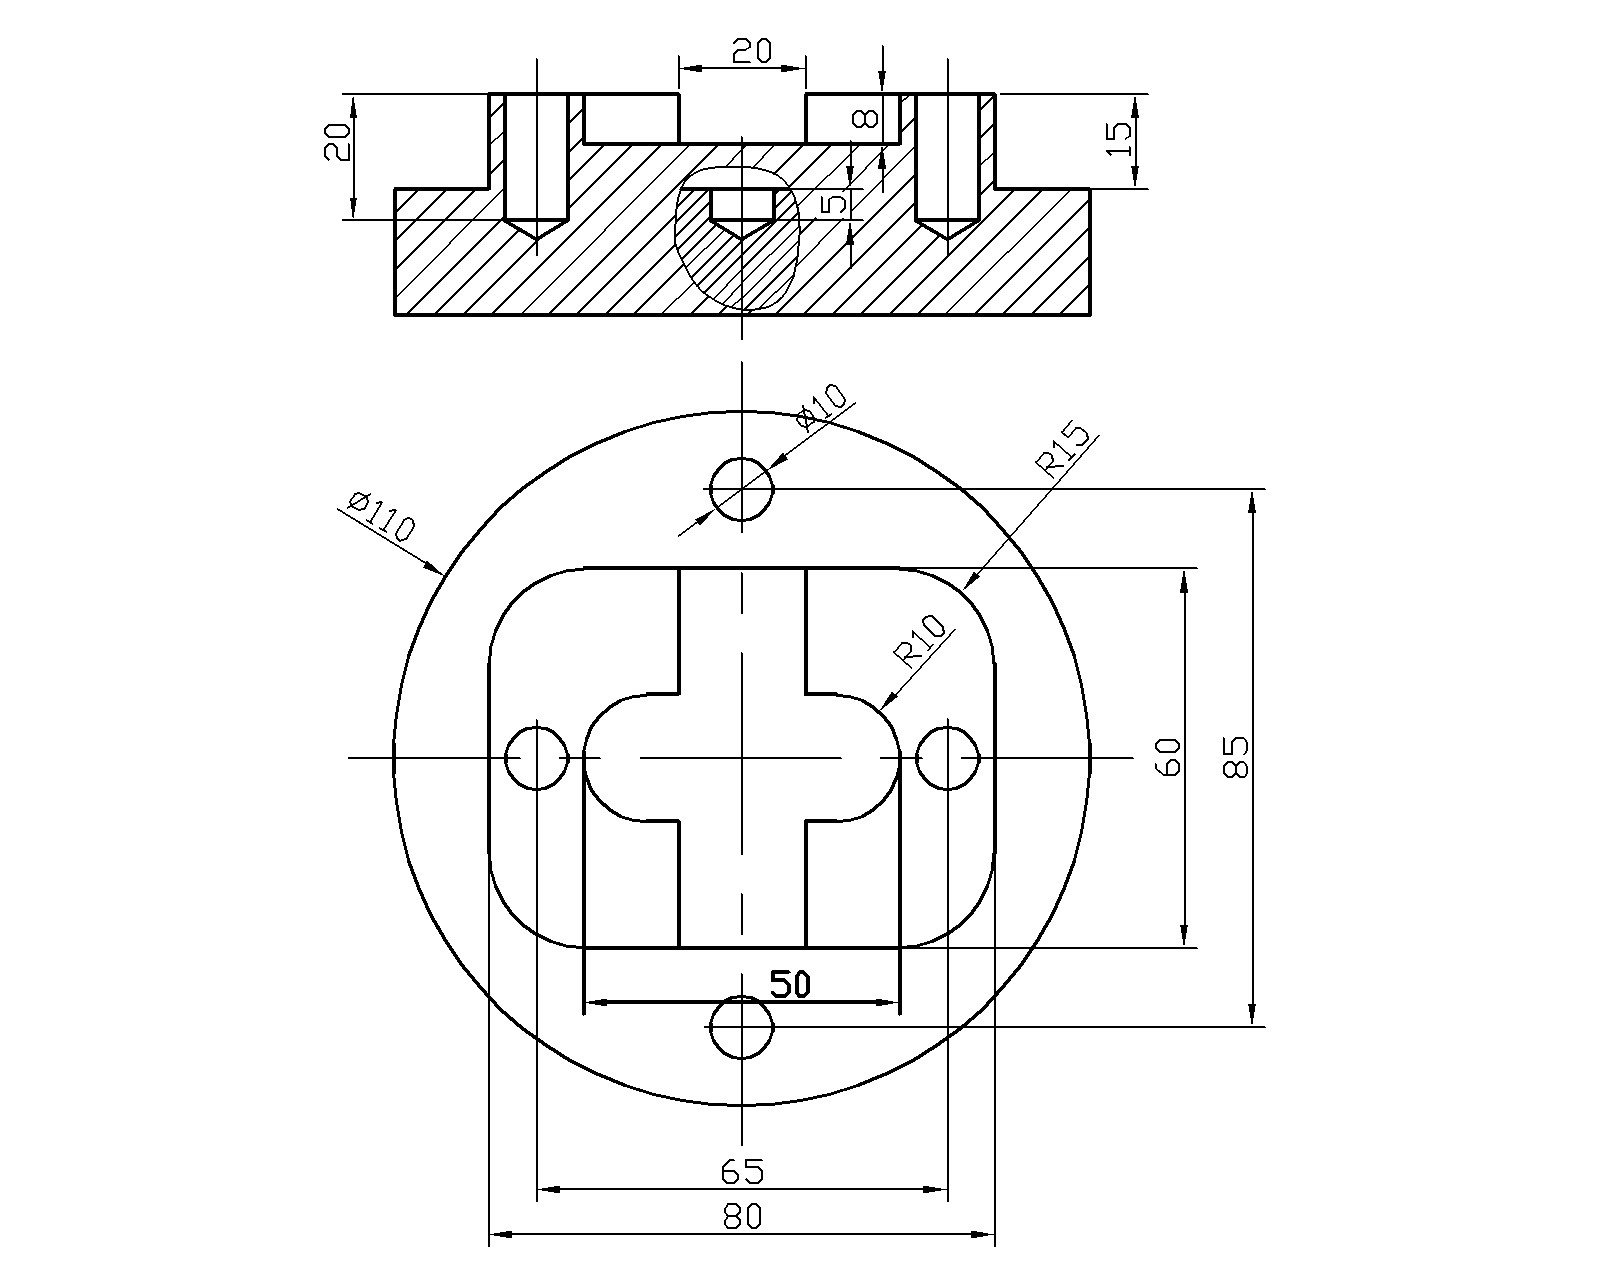
\includegraphics[width=0.6\linewidth,trim=250 10 250 10,clip]{image/1.jpg}
%	\caption{刀补实例}
	\label{fig:1}
\end{figure}

工艺:  

\newpage 程序: \newpage
程序:

	\end{enumerate} 
	\end{spacing}
\end{document}